\chapter{直线和平面}
\section{空间图形}
在初中几何课中,我们讨论的几何图形和几何问题,主
要局限在一个平面上。然而,我们生活着的现实世界却是具
有长、宽、高的所谓“三维空间”。而平面只是我们生活空
间的某个断面。我们日常所见的形体,如桌椅、房屋、球、
漏斗等等,它们并不局限在一个平面上,都是立体的。为了
精确地认识这些实际存在的形体,以便为我们的生产和生活
服务,我们必须学习有关空间图形的知识。

我们知道平面图形是同一平面上的点的集合,而\textbf{空间图
形却是不全在同一平面上的点的集合}。例如正方体、三棱
锥、圆柱、球等都是空间图形。空间图形也叫立体图形。我
们将在平面几何知识的基础上,来研究空间图形的性质、画
法以及有关的计算和应用。

\begin{figure}[htp]
    \centering
\begin{tikzpicture}[>=latex, scale=.5]
\begin{scope}
\tkzDefPoints{0/0/A, 3/0/B, -1/1/D, 0/3/A'}
\tkzDefPointsBy[translation= from A to D](B){C}
\tkzDrawSegments(A,B A,D)
\tkzDefPointsBy[translation= from A to A'](B,C,D){B',C',D'}
\tkzDrawPolygon(A',B',C',D')
\tkzDrawSegments(A,B A,D)
\tkzDrawSegments(A,A' B,B' D,D')
\tkzDrawSegments[dashed](C,B C,D C,C')
\node at (1,-1){立方体};

\end{scope}
\begin{scope}[xshift=5cm]
    \tkzDefPoints{-.5/1/A, 3.5/1/B, .8/0/C, 1.5/4/D}
\tkzDrawPolygon(A,C,B,D)
\tkzDrawSegments(C,D)
\tkzDrawSegments[dashed](A,B)
\node at (1.5,-1){三棱锥};
\end{scope}
\begin{scope}[xshift=10cm]
\tkzDefPoints{0/.5/A, 4/.5/B, 4/3.5/C, 0/3.5/D}
\draw(A) arc [start angle =-180, end angle =0, x radius=2, y radius=.5];
\draw[dashed](A) arc [start angle =180, end angle =0, x radius=2, y radius=.5];
\draw(D) arc [start angle =-180, end angle =0, x radius=2, y radius=.5];
\draw(D) arc [start angle =180, end angle =0, x radius=2, y radius=.5];
\node at (2,-1){圆柱};
\tkzDrawSegments(A,D B,C)
\end{scope}

\begin{scope}[xshift=15cm, yshift=2cm]
\tkzDefPoints{2.828/0/A, -2+2.828/0/B}
\tkzDefPoint(45:2){C}
\tkzDefPoint(-45:2){D}
\draw(A) circle (2);
\draw(B) arc [start angle =-180, end angle =0, x radius=2, y radius=.5];
\draw[dashed](B) arc [start angle =180, end angle =0, x radius=2, y radius=.5];
\draw[dashed,rotate=-45](C) arc [start angle =-180, end angle =0, x radius=2, y radius=.5];
\draw[rotate=-45](C) arc [start angle =180, end angle =0, x radius=2, y radius=.5];
\draw[dashed,rotate=45](D)  arc [start angle =-180, end angle =0, x radius=2, y radius=.5];
\draw[rotate=45](D) arc [start angle =180, end angle =0, x radius=2, y radius=.5];
\node at (3,-3){球};
\end{scope}

\end{tikzpicture}   
    \caption{}
\end{figure}

空间图形是在平面上(纸上)画出来的表示立体的图。
如在图1.1中,各图都表示出了某种立体。这种图形叫直
观图。除了用直观图表示立体以外,还有其他表示立体的方
法,如展开图和投影图等等。下面我们作些简要的介绍。

\subsection{直观图}
\subsubsection{水平放置的平面图形的画法}
当我们把一个正方形和圆放置在水平位置观察时,我们
的视觉会产生一些变化,总觉得它们像平行四边形和椭圆。
它们会变成怎样的平行四边形和椭圆呢?由于观察的角度不
同,会有不同的形状,这就涉及到了水平平面图形的画法问
题,下面就是较常用的两种画法。

第一种画法

\begin{example}
    画正方形的直观图。
\end{example}

\begin{figure}[htp]
    \centering
    \begin{tikzpicture}[>=latex,scale=1.5]
     \begin{scope}
\draw[<->](1.5,0)node[right]{$X$}--(0,0)--(0,1.5)node[right]{$Y$};
\draw(0,0)node[below]{$A$}--(1,0)node[below]{$B$}--(1,1)node[right]{$C$}--(0,1)node[left]{$D$};
\node at (.8,-.5,0){$(1)$};
\end{scope}   
\begin{scope}[xshift=3cm, x={(0:1cm)},y={(45:.5cm)},z={(90:1cm)}]
    \draw[<->](2,0,0)node[right]{$X'$}--(0,0,0)--(0,2,0)node[right]{$Y'$};
    \draw(0,0,0)node[below]{$A'$}--(1,0,0)node[below]{$B'$}--(1,1,0)node[right]{$C'$}--(0,1,0)node[left]{$D'$};
    \node at (1.5,-1.414,0){$(2)$};
    \end{scope}      
    \end{tikzpicture}
    \caption{}
\end{figure}

\textbf{画法}
\begin{enumerate}
    \item 在正方形$ABCD$上,分别取$AB$、$AD$为$X$轴
和$Y$轴,它们互相垂直于$A$点。

画对应的$X'$轴和$Y'$轴,使$\angle X'A'Y'=45^{\circ}$.
\item 在$X'$轴上截取$A'B'=AB$, 在$Y'$轴上截取
$A'D'=\frac{1}{2}AD$

\item 以$A'B'$、$A'D'$为邻边画平行四边形
$A'B'C'D'$就是正方形$ABCD$的直观图。(图1.2)。
\end{enumerate}

\begin{example}
    画正五边形的直观图。
\end{example}


\begin{figure}[htp]
    \centering
    \begin{tikzpicture}[>=latex,scale=1.2]
     \begin{scope}
\draw[<-](0,4)node[right]{$Y$}--(0,-.5); 
\draw[->](-2,0)--(2,0)node[right]{$X$};
\draw(-1,0)node[below]{$A$}--(1,0)node[below]{$B$}--(1.62,1.9)node[right]{$C$}--(0,3.08)node[right]{$D$}--(-1.62,1.9)node[left]{$E$}--(-1,0);
\draw[dashed](-1.62,1.9)--(-1.62,0)node[below]{$E_1$};
\draw[dashed](1.62,1.9)--(1.62,0)node[below]{$C_1$};
\node at (.25,-.25){$O$};
\node at (0,-1){$(1)$};
\end{scope}   
\begin{scope}[xshift=5cm, x={(0:1cm)},y={(45:.5cm)},z={(90:1cm)}]
    \draw[<-](0,6)node[right]{$Y'$}--(0,-1); 
    \draw[->](-2,0)--(3,0)node[right]{$X'$};
    \draw(-1,0)node[below]{$A'$}--(1,0)node[below]{$B'$}--(1.62,1.9)node[right]{$C'$}--(0,3.08)node[right]{$D'$}--(-1.62,1.9)node[left]{$E'$}--(-1,0);
    \draw[dashed](-1.62,1.9)--(-1.62,0)node[below]{$E'_1$};
    \draw[dashed](1.62,1.9)--(1.62,0)node[below]{$C'_1$};
    \node at (.25,-.5){$O'$};
    \node at (1,-2.828,0){$(2)$};
    \end{scope}      
    \end{tikzpicture}
    \caption{}
\end{figure}

\textbf{画法}
\begin{enumerate}
    \item 取正五边形$ABCDE$的$AB$所在直线为$X$轴,
    取$AB$的中垂线为$Y$轴($Y$轴必过$D$点),两轴交于$O$点.
    (图1.3(1))

    画对应的$X'$轴,$Y'$轴,使$\angle X'O'Y'=45^{\circ}$
    \item 作$CC_1\bot X$轴于$C_1$, 作$EE_1\bot X$轴于$E_1$, 在
    $X'$轴上取$A'B'=AB$, 且使$O'$为$A'B'$中点,并在$X'$轴
    上分别取$C'_1$点和$E'_1$点,使$O'C'_1=OC_1$, $O'E'_1=OE_1$.
    \item 在$Y'$轴上截取$O'D'=\frac{1}{2}OD$, 并引$E'_1E'\parallel
    O'Y'$, 且使$E'_1E=\frac{1}{2}E_1E$, 引$C_1'C'\parallel O'Y'$, 且使
    $C'_1C'=\frac{1}{2}C_1C$.
    \item 连结$A'E'$、$E'D'$、$D'C'$、$C'B'$, 则五边
    形$A'B'C'D'E'$就是正五边形$ABCDE$的直观图。(图
    1.3(2))
\end{enumerate}

通过上面例题,我们可以得出这种画法的规则如下:
\begin{enumerate}
\item 在图形上取互相垂直的$X$轴、$Y$轴,并画出与之
对应的$X'$轴,$Y'$轴,使$\angle X'O'Y'=45^{\circ}$(或$135^{\circ}$), $X'$
轴和$Y'$轴所确定的平面表示水平平面。
\item 图形中平行于$X$轴或$Y$轴的线段(包括在轴上的
线段)分别画成平行于$X'$轴和$Y'$轴的线段。
\item 平行于$X$轴的线段,长度不变;平行于$Y$轴的线
段,长度变为原来的一半。
\end{enumerate}

第二种画法

\begin{example}
   画圆的直观图 

   圆的直观图是一个椭圆,常采用如下近似画法:
\begin{enumerate}
    \item 取$\odot O$的一对互相垂直的直径$AB$, $CD$分别为$X$
轴、$Y$轴,并画出对应的$X'$轴、$Y'$轴,使$\angle X'O'Y'=120^{\circ}$.
\item 在$O'X'$上取$O'A'=OA$, 并取$A'$关于$O'$的对称
点$B'$, 然后在$O'Y'$轴上取$O'C'=OC$, 并取$C'$关于$O'$的对
称点$D'$.
\item 过$A'$、$B'$作$O'Y'$的平行线,过$C'$、$D'$作$O'X'$
的平行线,所作四条直线交出一个菱形,设$E$、$F$是菱形关
于$O'$点对称的顶点。
\item 连$ED'$, $FA'$, 交于$G$; 连$EB'$、$FC'$交于$H$.
\item 以$E$为心,以$ED'$为半径,作$\wideparen{D'B'}$, 以$F$为心,
以$FA'$为半径作$\wideparen{A'C'}$, 以$G$为心,以$GA'$为半径作$\wideparen{D'A}$,
以$H$为心,以$HC'$半径作$\wideparen{B'C'}$, 则此四弧连接成一个近似椭
圆.(图1.4(2))
\end{enumerate}

\begin{figure}[htp]
    \centering
    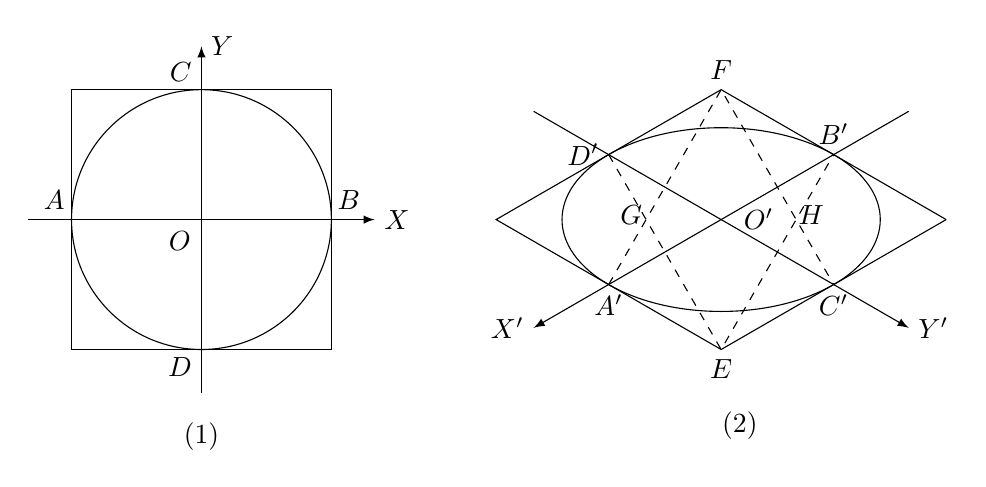
\begin{tikzpicture}[>=latex,scale=1.1]
     \begin{scope}
\draw[<-](0,2)node[right]{$Y$}--(0,-2); 
\draw[->](-2,0)--(2,0)node[right]{$X$};
\draw(-1.5,-1.5)--(-1.5,1.5)--(1.5,1.5)--(1.5,-1.5)--(-1.5,-1.5);
\draw (0,0) circle (1.5);
\node at (-1.7,0)[above]{$A$};
\node at (1.7,0)[above]{$B$};
\node at (0,1.7)[left]{$C$};
\node at (0,-1.7)[left]{$D$};
\node at (-.25,-.25){$O$};
\node at (0,-2.5){$(1)$};
\end{scope}   
\begin{scope}[xshift=6cm, x={(-150:1cm)},y={(150:1cm)}]
    \draw[->](0,2.5)--(0,-2.5)node[right]{$Y'$}; 
    \draw[->](-2.5,0)--(2.5,0)node[left]{$X'$};
    \draw(-1.5,-1.5)--(-1.5,1.5)--(1.5,1.5)--(1.5,-1.5)--(-1.5,-1.5);
    \draw (0,0) circle (1.5);
    \node at (-1.5,0)[above]{$B'$};
    \node  at (1.5,0)[below]{$A'$};
    \node  at (0,1.5) [left]{$D'$};
    \node  at (0,-1.5)[below]{$C'$};
    \node  at (-.25,-.25){$O'$};
    \node  at (.55,.65){$G$};
    \node  at (-.65,-.55){$H$};
    \draw[dashed](0,1.5)--(1.5,-1.5)node[below]{$E$}--(-1.5,0);
    \draw[dashed](1.5,0)--(-1.5,1.5)node[above]{$F$}--(0,-1.5);
    \node at (2.25,-2.5){$(2)$};
    \end{scope}      
    \end{tikzpicture}
    \caption{}
\end{figure}

从上述画法中,我们看出圆的中心$O$, 变成了椭圆的中
心$O'$, 圆的一对互相垂直的直径(如$AB$、$CD$)变成椭圆
的一对直径(如$A'B'$, $C'D'$),它们叫做椭圆的共轭直
径,实际上如果知道了一对椭圆的共轭直径,就可以把椭圆
近似地画出来了。

更省事的办法是用椭圆模板(图1.5)经过椭圆的一对
共轭直径端点来画椭圆。
\begin{figure}[htp]
    \centering
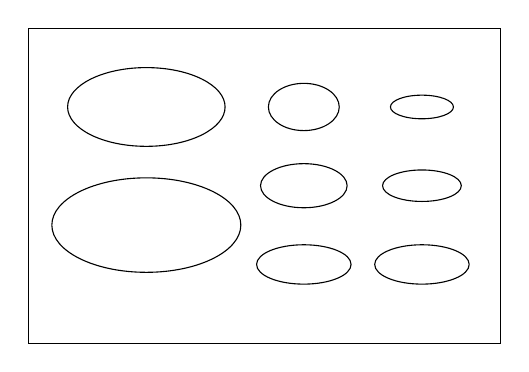
\begin{tikzpicture}[>=latex]
\draw(0,0) rectangle (6,4);
\draw(1.5,1.5) ellipse[x radius=1.2, y radius=.6];
\draw(1.5,3) ellipse[x radius=1, y radius=.5];
\draw(3.5,3) ellipse[x radius=.45, y radius=.3];
\draw(3.5,2) ellipse[x radius=.55, y radius=.28];
\draw(3.5,1) ellipse[x radius=.6, y radius=.25];
\draw(5,3) ellipse[x radius=.4, y radius=.15];
\draw(5,2) ellipse[x radius=.5, y radius=.2];
\draw(5,1) ellipse[x radius=.6, y radius=.25];
\end{tikzpicture}
    \caption{}
\end{figure}

从上例中可以看到:\textbf{第二种画法与第一种画法不同的,只
是$\angle X'O'Y'=120^{\circ}$;并且平行于$Y$轴的线段的长度不变}.

注意:直观图画好以后,要擦去辅助线。
\end{example}

\begin{ex}
\begin{enumerate}
\item 任意画一个三角形,然后用两种方法画出它们的直观图。
\item 任意画一个长方形,然后用两种方法画出它们的直观图。
\item 已知椭圆的一对共轭直径$AA'$、$BB'$, 近似地画出这个
椭圆。
\item 画一个边长为1.5cm的正六边形,然后用两种方法画出
它的直观图。
\end{enumerate}

(注意:以上练习只要求精确而美观地画出图形,不要
求写作法。)
\end{ex}

\subsubsection{空间形体的直观图}
\begin{example}
    画一个长、宽、高分别为3cm, 2cm和1.5cm的长
方体的直观图。
\end{example}

第一种画法:
\begin{enumerate}
    \item 在水平平面上画$X'$轴和$Y'$轴,两轴交于$O'$点,
    且使$\angle X'O'Y'=135^{\circ}$.
    \item 在$O'X'$上取$O'P'=1$cm, 在$O'Y'$上取$O'S'=
    3$cm, 作$S'R'\parallel O'X'$, $P'R'\parallel O'Y'$, 则平行四边形$O'P'R'S'$
    为已知长方体的底面的直观图。
    \item 过$O'$点作$Z'$轴垂直于$Y'$轴,并在$O'Z'$上取$OO'
    =1.5$cm, 过$P'$、$R'$、$S'$分别作$PP'\parallel O'Z'$, $RR' \parallel O'Z'$,
    $SS'\parallel O'Z'$, 并且,$PP'=RR'=SS'=1.5$cm.
    \item 连$OP$、$PR$、$RS$、$SO$, 则$PRSO-P'R'S'O'$
    为已知长方体的直观图。(图1.6)    
\end{enumerate}

\begin{figure}[htp]
    \centering
    \begin{tikzpicture}[>=latex]
 \tkzDefPoints{0/0/O', 3/0/S', 2.25/-.75/R', -.75/-.75/P', 0/1.5/O}
\tkzDefPointsBy[translation = from O' to O](S',P',R'){S,P,R}
\tkzDrawPolygon(P,R,S,O)
\tkzDrawSegments[dashed](O,O' O',P' O',S')
\tkzDrawSegments(P',R' R',S' P,P' R,R' S,S')
\draw[->](O)--(0,2.5)node[right]{$Z'$};
\draw[->](S')--(4,0)node[right]{$Y'$};
\tkzLabelPoints[above left](P,R,S,O)
\tkzLabelPoints[below right](P',R',S',O')       
\draw[->](P')--(-1.5,-1.5)node[right]{$X'$};
    \end{tikzpicture}
    \caption{}
\end{figure}

第二种画法
\begin{enumerate}
    \item 作$\angle X'O'Y'=120^{\circ}$, 并取$X'$轴和$Y'$轴的对称
    轴$Z'$轴为铅直线。
    \item 作已知长方体底面的直观图$O'P'R'S'$; 在
    $O'Z'$上取$OO'=1.5$cm.
    \item 分别过$P'$、$R'$、$S'$作$O'Z'$的平行线$PP'$、$RR'$、
    $SS'$、并使$PP'=RR'=SS'=OO'$.
    \item 连结$OP$、$PR$、$RS$、$SO$, 则$OPRS-O'P'R'S'$为已知长方体的直观图。(图1.7)
\end{enumerate}

\begin{figure}[htp]
    \centering
    \begin{tikzpicture}[>=latex, scale=.9]
\tkzDefPoints{0/0/O', 0/1.5/O}
\tkzDefPoint(-150:2){P'} \tkzDefPoint(-30:3){S'}
\tkzDefPointsBy[translation = from O' to O](S',P'){S,P}
\tkzDefPointsBy[translation = from O' to P'](S'){R'}
\tkzDefPointsBy[translation = from O to P](S){R}
\tkzDrawPolygon(O,S,R,P)
\tkzDrawSegments[dashed](O,O' O',P' O',S')
\tkzDrawSegments(P',P R',R  S,S' P',R' R',S')
\tkzLabelPoints[below](P', R',S',O')
\tkzLabelPoints[above](P,R,S)        
\tkzLabelPoints[above right](O) 
\draw[->](O)--(0,2.5)node[right]{$Z'$};  
\draw[->](P')--(-150:3)node[right]{$X'$};
\draw[->](S')--(-30:4)node[right]{$Y'$};
    \end{tikzpicture}
    \caption{}
\end{figure}

通过例1.4我们看到,画空间形体的直观图规则是在平面
图形的直观图画法的基础上发展起来的。\textbf{它多了一个$Z'$轴,
并且平行于$Z'$轴的线段的平行性和长度都不变。在第一种
画法中,$O'X'$, $O'Y'$, $O'Z'$中,$\angle X'O'Y'=135^{\circ}$,
 $\angle Z'O'Y'=90^{\circ}$, 并使$O'Z'$在铅直位置。第二种画法中,
使$\angle X'O'Y'=\angle Y'O'Z'=\angle X'O'Z'=120^{\circ}$, 且使$O'Z'$轴
居铅直位置.在两种画法中,平行于$O'X'$轴和$O'Y'$轴的线
段长度的变化与画平面图形的直观图的规定相同}。在图中,
$X'O'Y'$表示水平平面,$Y'O'Z'$平面和$X'O'Z'$平面都表
示直立的平面。

\begin{example}
画底面半径为1.5cm,高为2.5cm的圆锥的直观图。

画法(略)见图1.8.
\begin{figure}[htp]
    \centering
    \includegraphics[scale=.5]{fig/1-8.png}
    \caption{}
\end{figure}
\end{example}

\begin{rmk}
\begin{enumerate}
    \item 如果要画的空间形体中的面上有圆,一般采用第二种画法来画它的直观图。
    \item 第二种画法画圆的直观图,所得椭圆,由于较宽,不直观,故有时用较扁的椭圆来代替。
\end{enumerate}
\end{rmk}


\begin{ex}
\begin{enumerate}
    \item 用第一种画法画一个棱长为3cm的立方体的直观图.
    \item 用第二种画法画一个长、宽、高分别为4cm, 3cm, 2cm的长方体的直观图。
    \item 画一个底面半径1cm, 高为2.5cm的圆柱的直观图。
    \item 右面是用第一种画法画出来表示某立体的直观图,试根据图上标的尺寸,用第二种画法画出这个立体的直观图来。(单位mm)
    \item 左图是用第二种画法画
    出的某立体的直观图,试根据图上标的尺寸(单位mm),用第一种画法画出该立体的直观图。
    \item 画棱长为4cm的正四面体的直观图\footnote{正四面体是由四个正三角形围成的封闭立体。}。
\end{enumerate}
\end{ex}



\begin{figure}[htp]
    \centering
    \begin{minipage}[t]{0.48\textwidth}
    \centering
        \includegraphics[scale=.5]{fig/ch1-4ti.png}
    \caption*{第4题}
    \end{minipage}
    \begin{minipage}[t]{0.48\textwidth}
    \centering
\includegraphics[scale=.5]{fig/ch1-5ti.png}
    \caption*{第5题}
    \end{minipage}
  \end{figure}

\subsection{投影图}

\subsubsection{二视图}

在上一节我们谈到了画空间形体的直观图的方法,这种方法,立体感觉强,但立体的各个侧面的形状和大小不容易一下看清楚,因此,也需要从不同的方向来观察空间形体,
从而画出表示该立体的方法,这种方法通常叫投影图法,是画机械和建筑物设计图的常用方法。

\begin{figure}[htp]
    \centering
\begin{tikzpicture}[>=latex]
\begin{scope}
    \tkzDefPoints{0/0/X, 5/0/Y, -2/-2/X', 0/3/X''}
\tkzDefPointsBy[translation= from X to X'](Y){Y'}    
\tkzDefPointsBy[translation= from X to X''](Y){Y''}    
\tkzDrawPolygon(X',Y',Y,Y'',X'',X)
\tkzLabelPoints[left](X)
\tkzLabelPoints[right](Y)
\tkzLabelPoint[below left](Y''){$\beta$}
\node at (-1.5,-1.75)[right]{$\alpha$};
\foreach \x in {-1,-0.2,1.5}
{
    \draw(1.5,\x) ellipse[x radius=.8, y radius=.3];
}
\tkzDefPoint(1.5-.8, -1){A'}
\tkzDefPoint(1.5+.8, -1){B'}
\tkzDefPoint(1.5-.8, -0.2){A}
\tkzDefPoint(1.5+.8, -0.2){B}
\tkzDefPoint(1.5-.8, 1.5){A''}
\tkzDefPoint(1.5+.8, 1.5){B''}
\tkzDefPoint(1.5+.8+1, 0){C'}
\tkzDefPointsBy[translation= from B' to C'](A',A,B,A'',B''){D',D,C,D'',C''}
\tkzDrawSegments[dashed](B,C B',C' B'',C'' A,D A',D' A'',D'')
\tkzDrawSegments[dashed](A,A' B,B' D',D'')
\tkzDrawSegments(A,A'' B,B'' C,D C'',D'' C',C'')

\fill[pattern=north east lines](1.5,-1)ellipse[x radius=.8, y radius=.3];
\fill[pattern=north east lines](D)rectangle(C'');

\draw(X)--(.7,0);
\draw(Y)--(2.3,0);
\draw[dashed](.7,0)--(2.3,0);
\end{scope}
\begin{scope}[xshift=6cm, scale=.7]
\tkzDefPoints{0/0/X, 5/0/Y, 0/4/X'', 5/4/Y'', 0/-3/X', 5/-3/Y'}
\tkzDrawPolygon(X',Y',Y'',X'')
\tkzLabelPoints[left](X)
\tkzLabelPoints[right](Y)
\draw[pattern=north east lines](2,-1.5)circle (1);
\draw[pattern=north east lines](1,1) rectangle (3,3.5);
\draw[dashed](1,1)--(1,-1.5);
\draw[dashed](3,1)--(3,-1.5);
\tkzDrawSegments(X,Y)
\node at (3,0)[above right]{基线};
\node at (3,2)[right]{主视图};
\node at (3,-1.5)[right]{俯视图};

\end{scope}
\end{tikzpicture}    
    \caption{}
\end{figure}

在图1.9(1)中,平面$\alpha$是水平平面,平面$\beta$是铅直平面这两个平面的交线是$XY$. 当圆柱垂直于水平面的时候,从正上方向下看,它是一个圆,也可以这样想,在这种观察下,圆柱被视线投影成一个圆,这个圆在$\alpha$平面上,如果我们从平面$\beta$的正前方看圆柱,就看到一个矩形,可设想,这时圆柱被从$\beta$平面正前方发出的视线投影成一个矩形,这个矩形在$\beta$平面上,我们把$\alpha$平面叫作\textbf{俯视图平面},$\beta$平面叫\textbf{主视图平面},$\alpha$和$\beta$的相交的直线$XY$叫\textbf{基线}。画在俯视图平面上的图叫\textbf{俯视图},画在主视图平面上的图叫\textbf{主视图},俯视图和主
视图合起来叫\textbf{二视图}。

通常把俯视图平面旋转$90^{\circ}$, 使俯视图和主视图画在同一个平面内,这就成了图1.9(2), 它表示的是圆柱的二视图。

\subsubsection{三视图}

有些立体图形只用二视图表示还不够,例如像图1.10(1)那样摆法的圆柱的俯视图和主视图都是矩形,这个二视图也可看成是长方体的二视图了,为了区别起见,我们再设一个与俯视图平面和主视图平面都垂直的第三个平面$\gamma$, 从左侧面看这个圆柱,它在$\gamma$平面上的投影是个圆。这第三个平面$\gamma$叫\textbf{左视图平面},在它上面画出的图叫\textbf{左视图}。

\begin{figure}[htp]
    \centering
\includegraphics[scale=.55]{fig/1-10-1.png}
    \includegraphics[scale=.55]{fig/1-10-2.png}
    \caption{}
    \end{figure}


主视图、俯视图、左视图三个视图统称三视图。
图1.10(2)就是圆柱的三视图。主视图和俯视图或主视图和左视图都叫二视图,二视图和三视图也叫投影图。

在制图中投影图是不画基线的,如图1.11表示的就是由一个大长方体上挖去一个小长方体后的三视图。

从上面的三视图中,可以清楚地看出三个视图的关系是:

\begin{verbatim}
    主俯两图长对正,
    主左两图高平齐,
    左俯两图宽相等
\end{verbatim}

了解上述三视图的基本关系,我们常常可以从二视图画出第三个视图。


\begin{figure}[htp]\centering
    \begin{minipage}[t]{0.48\textwidth}
    \centering
  \begin{tikzpicture}[>=latex, scale=1]
\draw(0,6) rectangle (2,4);
\draw(1,6)--(1,4);
\draw[dashed](0,4)--(0,2);
\draw[dashed](2,4)--(2,3);
\draw(0,1.4)--(0,2.2)--(1,2.2)--(1,3)--(2,3)--(2,1.4)--(0,1.4);
\draw[<->](0,3.5)--node[fill=white]{长}(2,3.5);
\draw[|<->|](2.4,3)--node[fill=white]{宽}(2.4,1.4);

\draw(3,6) rectangle (4.6,4);\draw(3.8,6)--(3.8,4);
\draw[dashed](2,4)--(3,4);
\draw[dashed](2,6)--(3,6);
\draw[<->](2.5,4)--node[fill=white]{高}(2.5,6);
\draw[|<->|](3,3.5)--node[fill=white]{宽}(4.6,3.5);
    \end{tikzpicture}
    \caption{}
    \end{minipage}
    \begin{minipage}[t]{0.48\textwidth}
    \centering
    \begin{tikzpicture}[>=latex, scale=.8]
\draw(0,0) rectangle (3,2); \node at (3,1)[right]{宽};
\draw(1,0)--(1,2);\draw(2,0)--(2,2);
    
\draw(0,3)--(0,6)--(1,6)--(1,5)--(2,5)--(2,6)--(3,6)--node[right]{高}(3,3)--(0,3);

\draw(4,6) rectangle (6,3);
\draw[dashed](4,5)--(6,5);
\node at (5,3)[below]{宽};\node at (6,4.5)[right]{高};

    \end{tikzpicture}
    \caption{}
    \end{minipage}
    \end{figure}


画出图1.12的左视图,并把这个三视图所表示的立体的直观图画出来。

画法:
\begin{enumerate}
    \item 画左视图(略解)。
    
    根据“主左两图高平齐”和“俯左两图宽相等”,先画出左视图轮廓是个矩形,再观察主俯两图细部,看出这个视图所表示的立体是在一个大长方体的顶部正中贯通前后挖去一个小长方体,这样就必须在左视图的轮廓矩形上加一条虚线,这就画出了左视图。
    \item 画直观图。
    
    我们采用第二种画法:(略解)
    
    首先分析观察视图所表示的组成形体的各部分形状,如1中所述的是一个大长方体挖去一个小长方体.然后,根据视图所给的长、宽、高画出这两个长方体的直观图,但要特别注意在视图上所反映的这两个长方体的相互位置关系,最后擦去不需要的线便得到视图所表示的立体的直观图。(见图1.13)
\end{enumerate}

\begin{figure}[htp]
    \centering
    \includegraphics[scale=.6]{fig/1-13.png}
    \caption{}
\end{figure}

\begin{ex}
    \begin{enumerate}
    \item 根据下列各二视图想想立体是什么形状,并画出它
    的直观图。
    \item 根据下列各投影图来想象立体的形状,并画出它们
    的直观图。
    
\end{enumerate}
\end{ex}

\begin{figure}[htp]
    \centering
\begin{tikzpicture}[>=latex]
\begin{scope}
\draw(0,0)node[left]{$X$}--(4,0)node[right]{$Y$};
\draw(1,1)--(3,1)--(2.6,2)--(1.4,2)--(1,1);
\draw(2,-1.5) circle (1);
\draw(2,-1.5) circle (.6);
\draw[dashed](1,1)--(1,-1.5);
\draw[dashed](1.4,2)--(1.4,-1.5);
\draw[dashed](2.6,2)--(2.6,-1.5);
\draw[dashed](3,1)--(3,-1.5);
\node at (2,-3){(1)};

\end{scope}
\begin{scope}[xshift=5cm]
\draw(0,0)node[left]{$X$}--(4,0)node[right]{$Y$};
\tkzDefPoints{1/.5/A, 3/.5/B, 2/2.3/C, 1/-.5/A', 3/-.5/B', 2/-2.3/C'}
\tkzDrawPolygon[thick](A,B,C)
\tkzDrawPolygon[thick](A',B',C')
\tkzDrawSegments[dashed](A,A' B,B' C,C')
\draw[thick](C)--(2,1.5);
\draw[thick](C')--(2,-1.5)--(B');
\draw[thick](2,-1.5)--(A');
\node at (2,-3){(2)};
\end{scope}

\end{tikzpicture}
    \caption*{第1题}
\end{figure}

\begin{figure}[htp]
    \centering
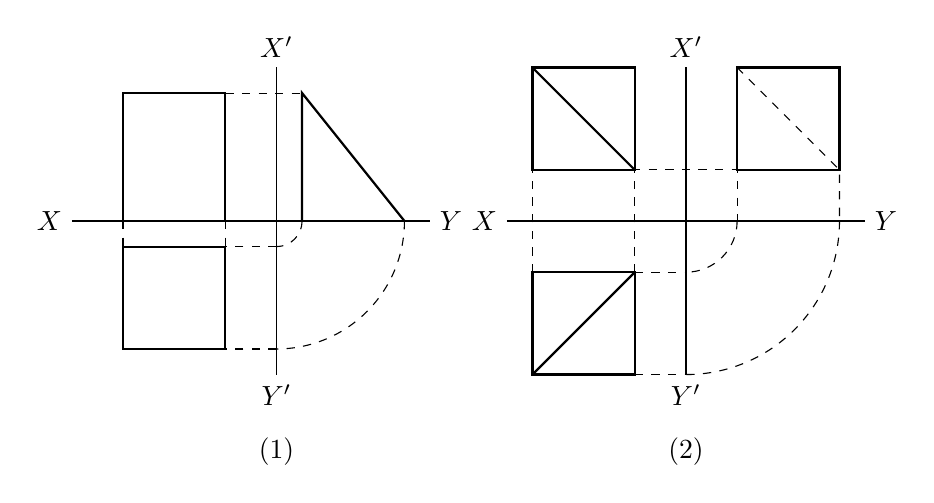
\begin{tikzpicture}[>=latex, scale=.65]
\begin{scope}
\draw(-4,0)node[left]{$X$}--(3,0)node[right]{$Y$};
\draw(0,-3)node[below]{$Y'$}--(0,3)node[above]{$X'$};
\draw[thick](-3,0) rectangle (-1,2.5);
\draw[thick](.5,0)--(.5,2.5)--(2.5,0);
\draw[thick](-3,-.5) rectangle (-1,-2.5);
\draw[dashed](-3,0)--(-3,-.5);
\draw[dashed](-1,0)--(-1,-.5);
\draw[dashed](0,-.5)--(-1,-.5);
\draw[dashed](0,-2.5)--(-1,-2.5);
\draw[dashed](-1,2.5)--(.5,2.5);
\node at (0,-4.5){(1)};
\draw[dashed](.5,0) arc (0:-90:.5);
\draw[dashed](2.5,0) arc (0:-90:2.5);


\end{scope}
\begin{scope}[xshift=8cm]
    \draw(-3.5,0)node[left]{$X$}--(3.5,0)node[right]{$Y$};
    \draw(0,-3)node[below]{$Y'$}--(0,3)node[above]{$X'$};
    \draw[thick](-3,1) rectangle (-1,3);
    \draw[thick](-3,-1) rectangle (-1,-3);
    \draw[thick](3,1) rectangle (1,3);
    \draw[thick](-3,3)--(-1,1);
    \draw[dashed](1,3)--(3,1)--(3,0);
    \draw[thick](-1,-1)--(-3,-3);
    \draw[dashed](-3,-1)--(-3,1);
    \draw[dashed](-1,-1)--(-1,1)--(1,1)--(1,0);
    \draw[dashed](-1,-1)--(0,-1);
    \draw[dashed](-1,-3)--(0,-3);
    \draw[dashed](1,0) arc (0:-90:1);
    \draw[dashed](3,0) arc (0:-90:3);
    \node at (0,-4.5){(2)};
\end{scope}


\end{tikzpicture}
    \caption*{第2题}
\end{figure}

\subsection*{习题1.1}
\begin{enumerate}
    \item 画出半径为2cm的球的三视图。
    \item 根据二视图,试
    补画出它的左视图,并画视图所表示的立体的直观图。
    \item 试回答下列二视图(1)—(4)中每一个是立
    体直观图(a)—(d)中的哪一个的视图。

    (注:(2)与(3)中的点划线表示的是该视图所表示的
    立体的轴线及中心线)

    \item 补全下列各视图的投影。
    \item 根据下列三视图,用两种方法画出它们所表示的立体直观图。
\end{enumerate}
















\section{集合运算}
\subsection{复习}
关于集合的初步知识,我们在初中几何中已经学过了,
现在简要地复习一下要点:

\subsubsection{集合}
通常我们把一些确定的、彼此不同的“事物”
作为一个整体考虑时,便说这个整体是一个\textbf{集合},这些事物叫做该集合的\textbf{元素}。

\begin{blk}{问题1}
    下列集合在空间表示什么图形?
\[\begin{split}
 A&=\{X| OX=5{\rm cm},\; O\text{点是三维空间的一个定点,
$X$是三维空间的点}\}\\
B&=\{P| OP<5{\rm cm},\; O\text{点是三维空间的一个定点,
$P$是三维空间的点}\}\\
C&=\{P| OP>5{\rm cm},\; O\text{点是三维空间的一个定点,
$P$是三维空间的点}\}   
\end{split}\]
\end{blk}

\subsubsection{集合关系}

\paragraph{包含关系}

如果集合$A$中的每一个元素也是集合$B$的元素,则称“$A$包含于$B$”或“$B$包含$A$”,也可以说$A$是$B$的子集。记作$A\subseteq B$, 或$B\supseteq A$. 

若$x\in A$, 则$x\in B$; 但$B$中至少有一个元素$y$不属于$A$, 则称$A$为$B$\textbf{真子集}。记作$A\subset B$或$B\supset A$.


\paragraph{相等关系}

如果两个集合$A,B$由共同的元素构成,我们说这两个集合相等,记作$A=B$. 

判定两个集合相等的方法是:若$A\subseteq B$且$B\subseteq A$, 则$A=B$. 

\begin{blk}{问题2}
    若$A\subset B$且$B\subset A$, 则$A$与$B$是否相等?为什么?
\end{blk}

\paragraph{空集、全集与补集}

不含有任何元素的集合叫做\textbf{空集},用$\emptyset$表示,空集是任何集合的子集。注意空集与零集合不同,零集合包含一个零元素,记作$\{0\}$, 而空集不含有任何元素.

我们把讨论对象所涉及的整个范围称作“全集”,用$I$表示。讨论的范围如果是整数,那么$I$就表示整数集。讨论的范围如果是实数,那么$I$就表示实数集。讨论的是三维空间,则$I$就表示三维空间。

设$A\subset I$, 则集合$\{x|x\in I,\; x\notin A\}$, 称为$A$的\textbf{补集},记作$\sim A$. 也可记作$\overline{A}$.

\begin{blk}{问题3}
\begin{enumerate}
    \item 若$I$为整数集,$A$是偶数集,则$\sim A$为什么
数集?
\item 若$I$为实数集,$A$为无理数集,则$\sim A$为什
么数集?
\end{enumerate}
\end{blk}

\paragraph{集合的“交”与“并”}

由集合$A$和集合$B$的共同元素所组成的集合称作集合$A$与$B$的\textbf{交集}.记作$A\cap B$,即
\[A\cap B=\{x|x\in A\text{ 且 }x\in B\}\]

由集合$A$的元素或集合$B$的元素合并而成的集合叫作$A$和$B$的\textbf{并集},记作$A\cup B$,即
\[A\cup B=\{x|x\in A\; \text{ 或 }\; x\in B\}\]

\begin{blk}{问题4}
    设$A=\{1,a,a^2\}$, $B=\{1,a,b\}$, 假定$a,b$都是实数,并且$A\cap B=\{1, 3\}$, $A\cup B=\{1,a,2a,3a\}$, 求
$a$和$b$的值分别是多少?
\end{blk}


\subsection{集合运算}

我们学过的集合的“交”、“并”、“补”都是集合的运算。

我们学过的数的运算是有算律的,那么集合的运算有什么算律呢?

我们很容易看出以下的事实成立:

\begin{blk}{}
\begin{itemize}
    \item $    A\cap A=A,\qquad     A\cup A=A$
\item $    A\cap I=A,\qquad    A\cup I=I$
\item $    A\cap \emptyset=\emptyset,\qquad  A\cup \emptyset=A$
\item $    A\cap B\subset A \quad \text{且}\quad A\cap B\subset B$
\item $A\subset A\cup B \quad \text{且}\quad B\subset A\cup B$
\item $A\cup \bar{A}=I,\qquad A\cap \bar{A}=\emptyset,\qquad \overline{\bar{A}}=A$    
\end{itemize}
\end{blk}

我们把$A\cap \bar{B}$称作$A$与$B$的\textbf{差集},记作$A-B$, 即
\[A-B=\{x|x\in A \quad \text{且}\quad x\notin B\}\]

差集的维恩图如图1.14所示:
\begin{figure}[htp]
    \centering
\begin{tikzpicture}[scale=1.2]
\begin{scope}
    \draw(-2,0) rectangle (2,3);
\fill[pattern=north east lines](-.65,1.5) circle (.9);
\draw[fill=white](.7,1.5) circle (1);
\draw(-.65,1.5) circle (.9);
\node at (2,0)[above left]{$I$};
\node at (-.65,2.6){$A$};
\node at (.7,2.7){$B$};
\node at (-.9,1.5)[fill=white]{$A-B$};
\node at (0,-.5){(1)};
\end{scope}
\begin{scope}[xshift=5cm]
    \draw(-2,0) rectangle (2,3);
\draw[pattern=north east lines](-.5,1.5) circle (1.2);
\draw[fill=white](-.5,1.8) circle (.5);

\node at (2,0)[above left]{$I$};
\node at (-1,2.8){$A$};
\node at (-.5,1.8){$B$};
\node at (-.5,.8)[fill=white]{$A-B$};
\node at (0,-.5){(2)};
\end{scope}
\begin{scope}[yshift=-4cm]
    \draw(-2,0) rectangle (2,3);
\draw[pattern=north east lines](-.65,1.5) circle (.9);
\draw[fill=white](.9,1.5) circle (.4);
\draw(-.65,1.5) circle (.9);
\node at (2,0)[above left]{$I$};
\node at (-.65,2.6){$A$};
\node at (.9,2.2){$B$};
\node at (-.65,1.5)[fill=white]{$A-B$};
\node at (0,-.5){(3)};
\end{scope}
\begin{scope}[xshift=5cm, yshift=-4cm]
    \draw(-2,0) rectangle (2,3)node[below left]{$I$};
    \draw(-.5,1.5) circle (1.2);
    \draw(-.5,1.8) circle (.5);
\node at (2,0)[above left]{$A-B=\emptyset$};
\node at (-.5,1.8){$A$};
\node at (-.5,1){$B$};
\node at (0,-.5){(4)};
\end{scope}
\end{tikzpicture}
    \caption{}
\end{figure}

\begin{blk}
    {问题1}设$A=\{\text{等腰三角形}\}$,$B=\{\text{直角三角形}\}$,
    则$A-B$是由什么三角形组成的集合?
\end{blk}


\begin{blk}
     {问题2}如果$A$为有理数的集合,$B$为非负有理数的集合,
    那么$A-B$是什么集合?
\end{blk}

\begin{blk}
     {问题3}设$I$为全集,$A$为$I$的一个子集,则$I-A$是个什么集
    合?(参看下面的维恩图思考)
\end{blk}

由问题3可知:
\[I-A=I\cap \bar A=\bar A\]

由此可见:补集可以看作差
集的特殊情况。

\begin{figure}[htp]
    \centering
\begin{tikzpicture}
\draw[pattern= north east lines](0,3) rectangle (4,0)node[above left, fill=white]{$I$};
\draw[fill=white](2,1) circle (.7);
\node at (2,1){$A$};
\node at (2,2.5)[fill=white]{$I-A$};
\end{tikzpicture}
    \caption{}
\end{figure}


集合的交集、并集和差集三
种运算很类似于数的乘法、加法
和减法,例如在数的计算中有
\[3\x2=2\x 3,\qquad 3+2=2+3\] 
在集合的运算中相应地有\[A\cap B=B\cap A,\qquad  A\cup B=B\cup A\]
在数的计算中有:
\[3\x(2\x4)=(3\x2)\x4,\qquad 3+(2+4)=(3+2)+4\]
在集合的运算中相应地有
\[A\cap (B\cap C)=(A\cap B)\cap C,\qquad 
A\cup (B\cup C)=(A\cup B)\cup C\]
这由维恩图很容易直观地看出
来。我们把它们所具有的一些算律归结为如下定理:

\begin{blk}
{定理} 集合的交与并满足以下算律
\begin{enumerate}
\item 结合律:
\[\begin{split}
     (A\cap B)\cap C=A\cap (B\cap C)&\qquad \text{(交的结合律)}\\
     (A\cup B)\cup C=A\cup (B\cup C)&\qquad \text{(并的结合律)}
\end{split} \]
\item 交换律:
\[\begin{split}
    A\cap B=B\cap A&\qquad \text{(交的交换律)}\\
    A\cup B=B\cup A&\qquad \text{(并的交换律)}
\end{split} \]
\end{enumerate}
\end{blk}

\begin{proof}
    我们只证“并的结合律”,其余类似地由同学们
    自己证明。
\[\begin{split}
     x\in (A\cup B)\cup C &\quad \Rightarrow \quad x\in (A\cup B)\; \text{ 或 }\;  x\in C\\
     &\quad \Rightarrow \quad  (x\in A \; \text{ 或 }\;  x\in B)\; \text{ 或 }\;  x\in C  \\
     &\quad \Rightarrow \quad   x\in A\; \text{ 或 }\;  (x\in B\; \text{ 或 }\;  x\in C) \\
     &\quad \Rightarrow \quad  x\in A\; \text{ 或 }\;  x\in (B\cup C) \\
     &\quad \Rightarrow \quad  x\in A\cup (B\cup C)  
\end{split}\]
$\therefore\quad (A\cup B)\cup C\subseteq A\cup (B\cup C)$

同理可证:$A\cup (B\cup C)\subseteq (A\cup B)\cup C$

$\therefore\quad (A\cup B)\cup C=A\cup (B\cup C)$
\end{proof}



















\begin{example}
    
\end{example}
\begin{solution}
    
\end{solution}


\begin{example}
    
\end{example}

\begin{solution}
    
\end{solution}

\begin{example}
    
\end{example}
\begin{solution}
    
\end{solution}


\begin{example}
    
\end{example}

\begin{solution}
    
\end{solution}


\begin{example}
    
\end{example}

\begin{solution}
    
\end{solution}



\begin{example}
    
\end{example}

\begin{solution}
    
\end{solution}


\begin{example}
    
\end{example}

\begin{solution}
    
\end{solution}






\begin{example}
    
\end{example}



\begin{solution}
    
\end{solution}

\begin{example}
    
\end{example}




\begin{solution}
    
\end{solution}




\begin{example}
    
\end{example}

\begin{solution}
    
\end{solution}
\begin{example}
    
\end{example}


\begin{solution}
    
\end{solution}






\begin{example}
    
\end{example}
\begin{solution}
    
\end{solution}

\begin{example}
    
\end{example}

\begin{solution}
    
\end{solution}

\begin{example}
    
\end{example}

\begin{solution}
    
\end{solution}

\begin{example}
    
\end{example}
\begin{solution}
    
\end{solution}

\begin{solution}
    
\end{solution}

\begin{solution}
    
\end{solution}

\begin{solution}
    
\end{solution}

\begin{solution}
    
\end{solution}
\begin{example}
    
\end{example}

\begin{solution}
    
\end{solution}
\begin{example}
    
\end{example}

\begin{solution}
    
\end{solution}
\begin{example}
    
\end{example}


\begin{solution}
    
\end{solution}
\begin{example}
    
\end{example}

\begin{example}
    
\end{example}
\begin{example}
    
\end{example}





\subsection*{习题1.7}
\begin{enumerate}
    \item 在平面$\pi$的同侧有$A,B$两点,在$\pi$上求一点$P$, 使$AP+
    BP$达到极小。
    \item 在平面$\pi$外有两点$A,B$, 且直线$AB\nparallel \pi$, 在$\pi$在上求一
    点$P$, 使$|AP-BP|$达到极大。
    \item 试问一个正方体有几个对称面?一个长方体有几个对
    称面?
    \item 证明:任何过球心的平面都是球的对称面。
\end{enumerate}

\section{章末提示}

本章主要内容是研究了空间直线和平面的关系,这包括
直线与直线,直线与平面,平面与平面之间的相互关系,在
概括本章内容时,请注意以下几点:

\subsection{要抓住平行、垂直、夹角和距离的概念}

这些概念都可看成是由平面几何推广而来的。
\begin{enumerate}
\item 平行:在平面几何中只有两条直线互相平行的概念,
但在立体几何中已把这种概念推广到直线与平面的平行和平
面与平面的平行,要注意它们的区别和联系。
\item 夹角:在平面几何中只有平面上两条直线交角的概
念,但在空间却推广到了异面直线的夹角,以及直线与平面的
夹角和二面角。然而这些推广了的概念,却都依赖于平面上
的角。
\item 垂直:在平面几何中只定义了同一平面内的两条直
线互相垂直。但在空间,却推广到了两条异面直线的垂直,
直线与平面的垂直,以及平面和平面的垂直。垂直的概念虽
然作了种种推广,但其基础却仍是同一平面上两条直线的垂
直。
\item 距离:在平面几何中已经有了两点间距离,点到直
线的距离以及两条平行线间的距离,到了空间,距离的概念
就更复杂了,不仅有了异面直线的距离,还有点到平面的距
离,以及两个平行平面间的距离。距离的概念虽然逐步推
广,但最原始的依据仍是“两点间距离”。
\end{enumerate}

\subsection{要抓住几个最主要的定理}
\begin{blk}
    {定理1(关于平行的定理)}
\begin{enumerate}
\item 如果两个平行平面同时和第三个平面相交,那么它们
的交线平行。
\item 如果一条直线平行于平面内的一条直线,那么这条直
线和这个平面平行。
\item 如果相交的两条直线都平行于一个平面,那么这两条
相交直线所确定的平面也平行于这个平面。
\item 过平面外一点唯一存在一个平面和已知平面平行。
\item 平行于同一平面的两个平面平行。
\item 平行于同一直线的两条直线互相平行。
\end{enumerate}
\end{blk}




\begin{blk}
    {定理2(关于垂直的定理)}
在空间$V$中和相异两点$P$、$P'$距离相等的点的集合是一
个平面$\pi$, 它和$PP'$相交于$PP'$的中点$M$, 而且$PP'$和$\pi$上
的任何一条直线都垂直。
\end{blk}

\begin{blk}
{推论1} 设$\ell\cap \pi=M$, $\ell_1$、$\ell_2$是$\pi$中两条相交直线,则$\ell\bot\pi$
的充要条件是$\ell\bot \ell_1$且$\ell\bot \ell_2$.
\end{blk}

\begin{blk}
{推论2}
设$\ell_1\bot\pi$, 则$\ell_2\bot\pi$的充要条件是$\ell_1\parallel \ell_2$.
\end{blk}

\begin{blk}
{推论3}
设$\ell\bot \pi_1$, 则$\ell\bot \pi_2$的充要条件是$\pi_1\parallel \pi_2$.
\end{blk}

\begin{blk}
{推论4}
$\pi\bot \pi'$的充要条件是$\pi'$含有$\pi$的一条垂线。

\end{blk}

\begin{blk}
    {推论5(三垂线定理)}
    设$PM\bot \pi$于$M$, $MQ$, $\ell\subset \pi$, 
$\ell\bot MQ$, 则$PQ\bot \ell$.
\end{blk}

\begin{blk}
{推论6(三垂线定理的逆定理)}设$PM\bot \pi$于$M$, $MQ$, 
$\ell\subset \pi$, $\ell\bot PQ$, 则$\ell\bot MQ$.
\end{blk}

\begin{blk}
    {定义} 空间$V$对给定平面$\pi$的对称是一个具有下列性质
的映射$R_{\pi}:\; V\mapsto V$; 对于任何点$P\in V$, 它的像是$R_{\pi}(P)=P'$, 
线段$PP'$被平面$\pi$垂直平分。
\end{blk}

\begin{blk}
    {定理3} 上述定义的映射$R_{\pi}$是一个保距映射,即对$V$
中任给两点$P,Q$, 总有$d(R_{\pi}(P),R_{\pi}(Q))=d(P,Q)$.
\end{blk}

\subsection{要注意立体几何解题思考方法的特点}
解立体几何题主要思考方法是和平面几何取得联系,从
而利用平面几何的知识解决立体几何的问题。有的问题可归
为一平面上的问题来解决,如定理:经平面外一点唯一存在
一个平面和已知平面平行的证明中,就把直线$a,b,m$集中
到一个平面$\pi'$上,从而用平面几何的知识加以解决。有的问
题则需要一个以上的辅助平面,如图1.61之例2, 就利用了
两个相交的辅助平面来解决的。作辅助平面的方法取决于平
面的确定条件:
\begin{enumerate}
\item 经过不共线三点确定一个平面。
\item 一条直线和直线外一点确定一个平面。
\item 两条相交直线确定一个平面。
\item 两条平行直线确定一个平面。
\end{enumerate}

此外还可利用:
\begin{enumerate}
\item 过平面外一点作已知平面的平行平面。
\item 过平面上一条直线作已知平面的相交平面等。
\end{enumerate}

在论证和解决立体几何的问题中如果是平行、相交问
题,利用集合运算方法有时也比较方便,但要注意正确运用
集合运算的算律,有时还需要引入辅助集合,如平行线传递
性定理的证明,就利用了辅助集合$\pi_1$. 

另外在论证问题过程,如果直接证法不易解决就利用间
接证法,如反证法和同一法等,如图1.34的例1,就是利用
同一法使直线$c=a'=b'$解决的。而在平行平面的传递性中
又用反证法。反证法和同一法常常是解数学问题的有利工
具。

\subsection{要注意正确理解空间元素的关系和基本概念会正确
地画出立体图形}
要正确地掌握画一个立体的投影图及直观图的方法,并
在画图中灵活运用。在画直线及平面关系的图形时,常常把
直线与直线的关系,直线与平面的关系,通过平面与平面的
关系画出来。例如,“两条异面直线间的距离是2m, 它们所
成的角是$60^{\circ}$, 在这两条异面直线上各有一点,距它们所在
直线的公垂线的垂足都是10m, 求这两点间距离。”在解这
个题画图时,可有不同画法,有
的比较直观,有立体感,有的则没
有立体感。见图1.79的(1)、(2)、(3),
图(1)显然没有立体感;图(2)
由于有平面$\pi_1$, 立体感较强了,
但如何利用条件求解启发性不强,图(3)由于有了两个平面
$\pi_1$和$\pi_2$, 并使$\pi_1$和$\pi_2$交线上两点$P$、$Q$间的距离为异面直
线$\ell_1$和$\ell_2$的距离,这样$\ell_1$和$\ell_2$的夹角恰是二面角$\pi_1-PQ-\pi_2$的
平面角,这样不仅图形直观而且方便利用条件求解。

\begin{figure}[htp]
    \centering
    
    \caption{}
\end{figure}


\section*{复习题1}
\begin{enumerate}
    \item 下面各命题是否正确?正确的给以证明,错误的举出反
    例:
\begin{enumerate}[(1)]
\item 两条直线不平行则相交。
\item 两个平面有三个公共点,则这两个平面重合。
\item 直线$a\parallel$ 直线$b$, $b\subset$平面$M$, 则$a\parallel M$.
\item 直线$a\parallel$ 平面$M$, 则$a$平行于平面$M$内的任意直线。
\item 平面$M\parallel$ 平面$N$, 若直线$a\subset M$, 则$a\parallel N$.
\item 平面$M\parallel$ 平面$N$, 若直线$a\subset M$且直线$b\subset N$,则$a\parallel b$.
\item 平行于同一直线的两条直线平行。
\item 垂直于同一直线的两条直线平行。
\item 垂直于同一平面的两条直线平行。
\item 垂直于同一平面的两个平面平行。
\item 垂直于同一直线的两个平面平行。
\item 平行于同一平面的两条直线平行。
\item 平行于同一平面的两个平面平行。
\item 直线$a\bot$ 直线$b$, 直线$b\bot $直线$c$, 则$a\bot c$.
\item 直线$a\parallel$ 直线$b$, 直线$c\bot $直线$a$, 则$b\bot c$.
\item 直线$a\parallel$ 平面$M$, 直线$b\bot $直线$a$, 则$b\bot M$.
\item 直线$a\parallel $平面$Q$, 直线$b\parallel $平面$Q$, 若$a,b\subset M$, 则$M\parallel Q$.
\item 平面$Q\cap $平面$N=a$, 直线$b\subset Q$, $b\bot a$, 则$b\subset N$.
\item 过$A$点垂直于直线$a$的直线必在过$A$点垂直于$a$的平面
内。
\item 过点$A$平行于平面$a$的直线必在过点$A$平行平面$a$的平
面内。
\item 平面$\pi_1\bot $平面$\pi_2$, $\pi_1\cap \pi_2=a$, 直线$b\bot a$, 则$b\subset \pi_1$.
\item 两个角的边分别平行,则这两个角相等。
\item 直线$a\bot $直线$b$, 直线$a\bot $直线$c$, 若$b,c\subset $平面$\pi$, 则
$a\bot \pi$.
\item 过平面的一条斜线的斜线足,并且与这斜线的射影垂
直的直线,则它垂直于这斜线。
\item 两条直线确定一个平面。
\item 如果四个点不共面,那么它们中的任何三点都不共线。
\item 两条平行直线在同一平面上的射影互相平行。
\item 如果直线$a\parallel$ 直线$b$, 直线$b$和直线$c$是异面直线,那么
$a$和$c$是异面直线。
\end{enumerate}

\item 求证:两两相交但不过同一点的四条直线在同一平面
内。
\item 三平面两两相交出三条直线,求证:这三条直线交于一
点或互相平行。
\item 证明:分别过两异面直线中的一条直线,而与另一条平
行的两个平面互相平行。
\item 夹在两个平行平面间的两条线段$AB$、$CD$交于$P$, 已知:
$AP=18.9$cm, $BP=29.4$cm, $CD=57.5$cm, 求$CP$和$DP$
的长。
\item 直角三角形$ABC$所在的平面$\pi$外一点$P$到直角顶$C$的距离
为24cm, 到两直角边距离都是$6\sqrt{10}$cm, 求$P$点到平面$\pi$
的距离。
\item 在直二面角的棱上有两点$A,B$, $AC$, $BD$各在这个二
面角的一个面内,并且都垂直于棱,设$AB=8$cm, $AC
=6$cm, $BD=24$cm, 求$CD$的长.
\item 已知:共点的三条线段$OA$, $OB$, $OC$两点互相垂直,
且$OA=a$, $OB=b$, $OC=c$, 求$O$点到平面$ABC$的距离。
\item 一条长$2a$的线段夹在互相垂直的两个平面之间,它和两
个平面所成的角都是$30^{\circ}$, 求这条线段与这两个平面的
交线所成的角。




















\end{enumerate}